\documentclass[14pt]{beamer}
\usepackage{multimedia}

\usetheme[width=1.4cm]{PaloAlto}
\usecolortheme{default}
\useoutertheme{shadow} 

\usepackage[utf8]{inputenc}
\usepackage{booktabs,tabu}
\usepackage{adjustbox}
\usepackage{graphicx}
\usepackage{caption}
\graphicspath{{figs/}}
\DeclareGraphicsRule{.tif}{png}{.png}{`convert #1 `dirname #1`/`basename #1 .tif`.png}


%%%%%%%%%%%%%%%%%%%%
%%% BEGIN PYTHON %%%
%%%%%%%%%%%%%%%%%%%%

\usepackage{color}
\long\def\ans#1{{\color{blue}{\em #1}}}
\long\def\ansnem#1{{\color{blue}#1}}
\long\def\boldred#1{{\color{red}{\bf #1}}}

\usepackage{listings}
\usepackage{textcomp}
\renewcommand{\lstlistlistingname}{Code Listings}
\renewcommand{\lstlistingname}{Code Listing}

%%% Specific for python listings
\definecolor{gray}{gray}{0.5}
\definecolor{green}{rgb}{0,0.5,0}

\lstnewenvironment{python}[1][]{
\lstset{
language=python,
basicstyle=\tiny,
stringstyle=\color{red},
showstringspaces=false,
alsoletter={1234567890},
otherkeywords={\ , \}, \{},
keywordstyle=\color{blue},
emph={access,and,break,class,continue,def,del,elif ,else,%
except,exec,finally,for,from,global,if,import,in,i s,%
lambda,not,or,pass,print,raise,return,try,while},
emphstyle=\color{black}\bfseries,
emph={[2]True, False, None, self},
emphstyle=[2]\color{green},
emph={[3]from, import, as},
emphstyle=[3]\color{blue},
upquote=true,
morecomment=[s]{"""}{"""},
commentstyle=\color{gray}\slshape,
emph={[4]1, 2, 3, 4, 5, 6, 7, 8, 9, 0},
emphstyle=[4]\color{blue},
literate=*{:}{{\textcolor{blue}:}}{1}%
{=}{{\textcolor{blue}=}}{1}%
{-}{{\textcolor{blue}-}}{1}%
{+}{{\textcolor{blue}+}}{1}%
{*}{{\textcolor{blue}*}}{1}%
{!}{{\textcolor{blue}!}}{1}%
{(}{{\textcolor{blue}(}}{1}%
{)}{{\textcolor{blue})}}{1}%
{[}{{\textcolor{blue}[}}{1}%
{]}{{\textcolor{blue}]}}{1}%
{<}{{\textcolor{blue}<}}{1}%
{>}{{\textcolor{blue}>}}{1},%
%framexleftmargin=1mm, framextopmargin=1mm, frame=shadowbox, rulesepcolor=\color{blue},#1
framexleftmargin=1mm, framextopmargin=1mm, frame=single,#1
}}{}

%%%%%%%%%%%%%%%%%%
%%% END PYTHON %%%
%%%%%%%%%%%%%%%%%%


% remove navigation symbols
\setbeamertemplate{navigation symbols}{}
\setbeamerfont{page number in head/foot}{size=\fontsize{12}{12}}
\setbeamertemplate{footline}[frame number]

% make image sized to frame
\newcommand {\framedgraphic}[2] { % args = {frametitle}{image.ext}
    \begin{frame}{#1}
        \begin{center}
            \includegraphics[width=\textwidth,height=0.8\textheight,keepaspectratio]{#2}
        \end{center}
    \end{frame}
}

% This block will remove authornames and talk title from sidebar
\makeatletter
  \setbeamertemplate{sidebar \beamer@sidebarside}%{sidebar theme}
  {
    \beamer@tempdim=\beamer@sidebarwidth%
    \advance\beamer@tempdim by -6pt%
    \insertverticalnavigation{\beamer@sidebarwidth}%
    \vfill
    \ifx\beamer@sidebarside\beamer@lefttext%
    \else%
      \usebeamercolor{normal text}%
      \llap{\usebeamertemplate***{navigation symbols}\hskip0.1cm}%
      \vskip2pt%
    \fi%
}%
\makeatother




\begin{document}

\title{A TensorFlow Tutorial}  
\subtitle{Email Classification with Logistic Regression}
\author{Josh Meyer \inst{1} \and Michael Capizzi \inst{2}}
\institute{ \inst{1} University of Arizona \and \inst{2} PitchVantage}
\date{} 

\frame{\titlepage} 

\frame{\frametitle{Table of contents}\tableofcontents} 


\section{What's Going to Happen}

\frame{
Tonight we will...
\begin{itemize}
\item describe the basic TensorFlow structures
\item build a working example of text classification
\item point out places where \textit{other} TensorFlow "built-ins" apply {\footnotesize(optimizers, cost functions, etc)}
\item "hand-wave" liberally \\
{\footnotesize(when we don't want to get into it or don't know the answer)}
\end{itemize}
Tonight we will \textbf{not}...
\begin{itemize}
\item discuss details of NLP feature selection
\item discuss details of Machine Learning \\
{\footnotesize(linear algebra, backpropogation, etc.)}
\end{itemize}
}

\section{TensorFlow Structures}

\frame{\frametitle{}
  \centering
    \begingroup
    \fontsize{20pt}{20pt}\selectfont
    TensorFlow Structures
  \endgroup
  \begin{flushleft}
  tensor = \textit{n}-dimensional matrix
  \end{flushleft}
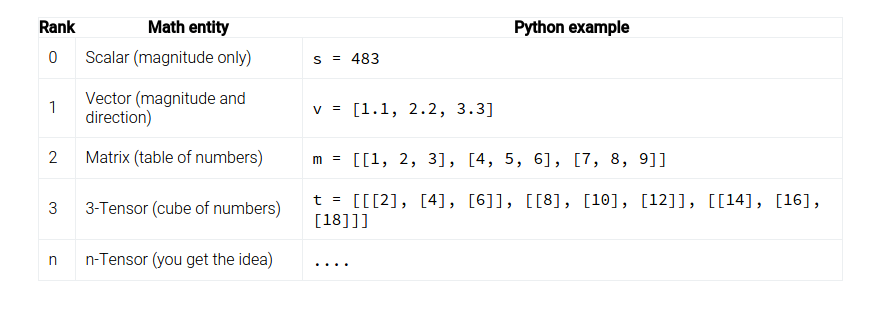
\includegraphics[width=\textwidth,height=0.9\textheight,keepaspectratio]{tensors.png}}

\begin{frame}[fragile]
\frametitle{TensorFlow Structures}
\begin{itemize}
\item{\textbf{constants}}: {\small \textit{never} changes its value(s)} \\
\begin{python}
c = tf.constant(2.0, name="constantC") #can be int, float, or tensor
\end{python}
\item{\textbf{placeholders}}: {\small shell into which tensors can be iteratively inserted} \\
\begin{python}
X = tf.placeholder(tf.float32, [None, 200], name="input")
\end{python}
\item{\textbf{variables}}: {\small value(s) can be updated}
\begin{python}
weights = tf.Variable(tf.random_normal([1, 200], name="weights"))
\end{python}
\item{\textbf{operations}}: {\small computations that will act on tensors}
\begin{python}
apply_weights_OP = tf.matmul(X, weights, name="apply_weights")
add_bias_OP = tf.add(apply_weights_OP, bias, name="add_bias")
activation_OP = tf.nn.sigmoid(add_bias_OP, name="activation")\end{python}
\end{itemize}
\end{frame}

\section{The Flow of TensorFlow}

\frame{\frametitle{}
  \centering
    \begingroup
    \fontsize{20pt}{20pt}\selectfont
    The \textit{Flow} \\
    of TensorFlow \\
  \endgroup
}


\framedgraphic{Initialize Weights \& Bias Terms}{1-initialization.png}

\begin{frame}[fragile]
  \begin{python}
#################
### VARIABLES ###
#################

# all values are randomly assigned:
# sqrt(6 / (numInputNodes + numOutputNodes + 1))

weights = tf.Variable(tf.random_normal([numFeatures,numLabels],
          mean=0,
          stddev=(np.sqrt(6/numFeatures+numLabels+1)),
          name="weights"))

bias = tf.Variable(tf.random_normal([1,numLabels],
       mean=0,
       stddev=(np.sqrt(6/numFeatures+numLabels+1)),
       name="bias"))


# INITIALIZE our weights and biases
init_OP = tf.initialize_all_variables()
  \end{python}
\end{frame}


\framedgraphic{Apply Weights to Features}{2-apply-weights.png}

\begin{frame}[fragile]
  \begin{python}
apply_weights_OP = tf.matmul(X, weights, name="apply_weights")
  \end{python}
\end{frame}


\framedgraphic{Add Bias to Weighted Features}{3-add-bias.png}

\begin{frame}[fragile]
  \begin{python}
add_bias_OP = tf.add(apply_weights_OP, bias, name="add_bias") 
  \end{python}
\end{frame}


\framedgraphic{Apply Sigmoid Activation}{4-apply-sigmoid.png}

\begin{frame}[fragile]
  \begin{python}
activation_OP = tf.nn.sigmoid(add_bias_OP, name="activation")
  \end{python}
\end{frame}


\framedgraphic{Full Computational Graph}{full-graph.png}



\frame{\frametitle{}
  \centering
  \begingroup
  \fontsize{12pt}{12pt}\selectfont
  Thank you! \\
  \endgroup
  \vspace{1cm}
}


\end{document}




%% \frame{\frametitle{The Flow of TensorFlow} 
%%   \begin{table}[H]
%%     \begin{adjustbox}{max width=\textwidth}
%%       \centering
%%       \begin{tabular}{lccc}
%%         \toprule
%%         \textbf{Study}       & \textbf{Languages}   & \textbf{Phonemic Feature}                       & \textbf{Best Predictor}\\
%%         \midrule
%%         Cutler et al. (1986, 1992)  & French-English       & Metrical Structure                            & Preference \\
%%         \bottomrule
%%       \end{tabular}
%%     \end{adjustbox}
%%   \end{table}
%% }
